\documentclass{standalone}
\usepackage[utf8]{inputenc}
\usepackage{newtxtext}
\usepackage{newtxmath}
\usepackage[italic]{hepnicenames}
\makeatletter\def\@shiftlen@anti@gen@bar{0mu}\makeatother
\usepackage[svgnames]{xcolor}
\usepackage{tikz-feynhand}


\begin{document}
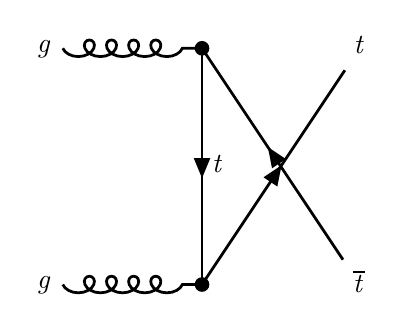
\begin{tikzpicture}
  \setlength{\feynhandlinesize}{1.0pt}
  \tikzfeynhandset{every dot={/tikz/color=Black},}
  \begin{feynhand}
    \vertex [particle, Black] (g1) at (-2.0, 1.5) {\Pg};
    \vertex [particle, Black] (g2) at (-2.0, -1.5) {\Pg};
    \vertex [particle, Black] (t1) at (2.0, 1.5) {\Pqt};
    \vertex [particle, Black] (t2) at (2.0, -1.5) {\Paqt};
    \vertex [dot, Black] (gt1) at (0.0, 1.5) {};
    \vertex [dot, Black] (gt2) at (0.0, -1.5) {};
    \propagator [gluon, Black] (g1) to (gt1);
    \propagator [gluon, Black] (g2) to (gt2);
    \propagator [fermion, Black] (gt2) to (t1);
    \propagator [fermion, Black] (gt1) to [edge label={\Pqt}, color=Black] (gt2);
    \propagator [fermion, Black] (t2) to (gt1);
  \end{feynhand}
\end{tikzpicture}
\end{document}
